\chapter{Vergleich der Cloud-Kosten}

Im folgenden Kapitel werden die monatlich anfallenden Cloud-Kosten \autocite{awsPricing} \autocite{gcpPricing} für die entwickelte Software am Standort Frankfurt verglichen. Die verwendeten Cloud-Dienste werden aus der Architektur extrahiert. Außerdem werden im Kapitel Anwendungsszenarien vorgestellt, um zu ermitteln, für welchen Fall welcher Dienst wirtschaftlicher ist.

\section{Kostenkategorien}

Der Unterabschnitt stellt die Kosten in unterschiedlichen Kategorien dar. Eine Kategorie kann aus einem oder mehreren Cloud-Diensten bestehen. Zu beachten ist, dass Amazon Cognito in der Preiskalkulation vernachlässigt wird. Da die erweiterten Sicherheitsfunktionalitäten von Amazon Cognito nicht genutzt werden, ist der Cloud-Dienst kostenlos. Seitens Firebase gibt es hier ebenfalls keine extra Kosten pro Nutzer.

\subsection{Hosting}

\begin{figure}%
    \centering
    \subfloat[\centering Gespeicherte Daten]{{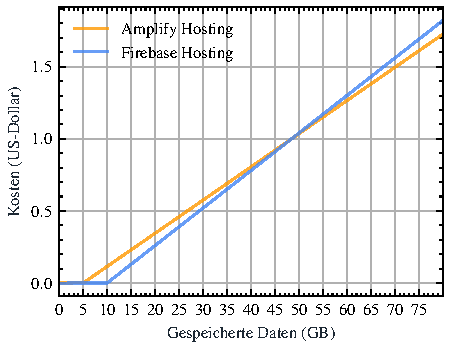
\includegraphics[width=6cm]{7_1_vergleich-cloud-kosten/hosting-stored-data.pdf} }}%
    \qquad
    \subfloat[\centering Übertragene Daten]{{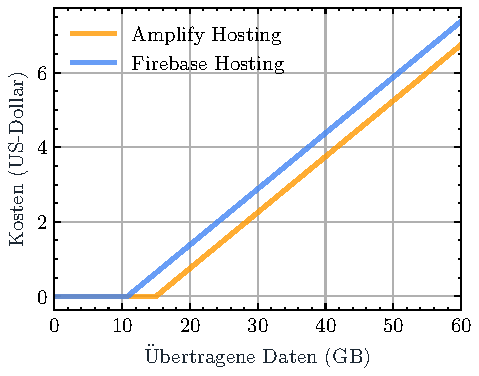
\includegraphics[width=6cm]{7_1_vergleich-cloud-kosten/hosting-transferred-data.pdf} }}%
    \caption{Kostenvergleich zwischen Amplify Hosting und Firebase Hosting}%
    \label{kostenvergleichHosting}%
\end{figure}

Amplify Hosting vs Firebase Hosting

Parameter:
- Gespeicherte Dateien
- Ausgelieferte Dateien

- Number of build minutes (nur AWS)


Amplify:
- Build minutes cost = Number of build minutes * 0,01 USD / min
- Data stored cost = Data stored per month GB * 0.023 USD / GB * mon
- Data served cost = Data served per month GB * 0.15 USD / GB * mon

Free tier:
5 GB stored per month
15 GB served per month

Firebase:
- Berechnung
    - Storage = $0.026/GB
    - Data transfer = $0.15/GB

Free tier:
- Storage 10 GB
- Data transfer: 10.8GB



\subsection{Serverless-Computing}

AWS Lambda inklusive AWS AppSync und Amazon EventBridge) mit Cloud Functions

AWS Lambda (x86)

  Paramater:
  - Number of requests: 10.000
  - Duration of each request: 300ms
  - Amount of memory allocated: 256MB

  Berechnung:
  - Compute Charges= Anzahl request * Durchschnittliche Request-Zeit * Durchschnittlich Benutzer Speicher * 0.0000166667 USD (1*sec*GB*USD/GBs)
  - Request Charges = Anzahl request * 0.0000002 USD

  Amazon EventBridge

  Parameter:
  - Payload Size: 10KB
  - Custom Events: 1 Million per Month

  Berechnung:
  - Event Costs: 1 Mio Custom Events x 0.000001 USD

  AppSync

  Parameter:
  - Query and Data Modification Operations per million
  - Average response size: 3KB

  Berechnung:
  - OperationCosts = Query and Data Modification Operations per million * $4.00 USD
  - Data Transfer Costs = Avg response size * Modifications * $0.09 USD /.GB



\subsection{Storage}

AWS S3 mit Cloud Storage

S3

Parameter
- S3 Standard Storage in GB
- PUT, COPY, POST, LIST Requests
- GET, SELECT Requests
- Inbound Data Transfer: Free
- Outbound Data Transfer: GB

Berechnung:
- S3 Standard Storage Costs: S3 Standard Storage in GB * 0.0245000000 USD
- S3 Standard PUT request costs: Number of PUT requests * 0.0000054 USD per request
- S3 Standard GET request costs: Number of GET requests * 0.00000043 USD per request
- Outbound Data Transfer:
    - 10240 GB x 0.09 USD per GB = 921.60 USD (next 10TB)
    - 40960 GB x 0.085 USD per GB = 3481.60 USD (next 40TB)
    - 102400 GB x 0.07 USD per GB = 7168.00 USD (next 100TB)
    - 999846400 GB x 0.05 USD per GB = 49992320.00 USD (larger than 150TB)





\subsection{Datenbank-Service}

DynamoDB mit Cloud Firestore

DynamoDB

Parameter:
- Data storage size in GB
- Average item size
- Writes
    - Standard writes vs Transactional writes: 100 / 0
    - Number of writes: 1000
- Reads
    - Eventually consistent vs Strongly vs Transactional: 100 / 0 / 0
    - Number of reads: 10 million per month
- On demand backup data storage

Berechnung:
- Data storage costs: Data storage size * 0.306 USD
- Write costs: Number of writes * 0.000001525 USD
- Read costs: Number of reads x 1 strongly consistent portion x 1 read request units for strongly consistent reads x 25 read request units needed per item = 7,850,000,000.00 read request units for strongly consistent reads * 0.000000305 USD
- Backup storage costs: On demand backup data storage x 0.1224 USD

\subsection{Videokonvertierung}

\begin{figure}
  \centering
  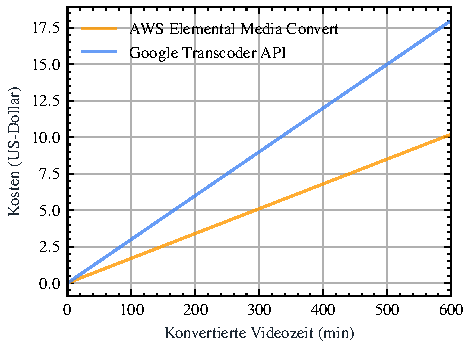
\includegraphics[width=0.75\columnwidth]{7_1_vergleich-cloud-kosten/transcoding.pdf}
  \caption{Kostenvergleich zwischen AWS Elemental Media Convert und Google Transcoder API}
  \label{KostenVideoTranscoding}
\end{figure}

AWS Elemental MediaConvert mit Google Transcoder API

AWS Elemental MediaConvert

Parameter:
- Tier: basic (Fix), Video-Codec: AVC, Single pass, HD, <= 30 FPS
- Output usage minutes per month

Berechnung:
- Outputs: Output usage minutes per month * 0.017 USD / minute


Google Transcoder API
- Parameter
    - Minutes HD conversion
- Berechnung
    - Price = Minutes * $0.030 USD / minute


\subsection{Zusammenfassung}

zusammenfassung aller dienste und wo welcher dienst günstiger ist

\section{Preisbeispiele}

- Szenarien 1 2 3 ggf. auch nur eins

TODO: Nutzungsprofile für die Anwendung definieren, damit der vergleich einfacher ist